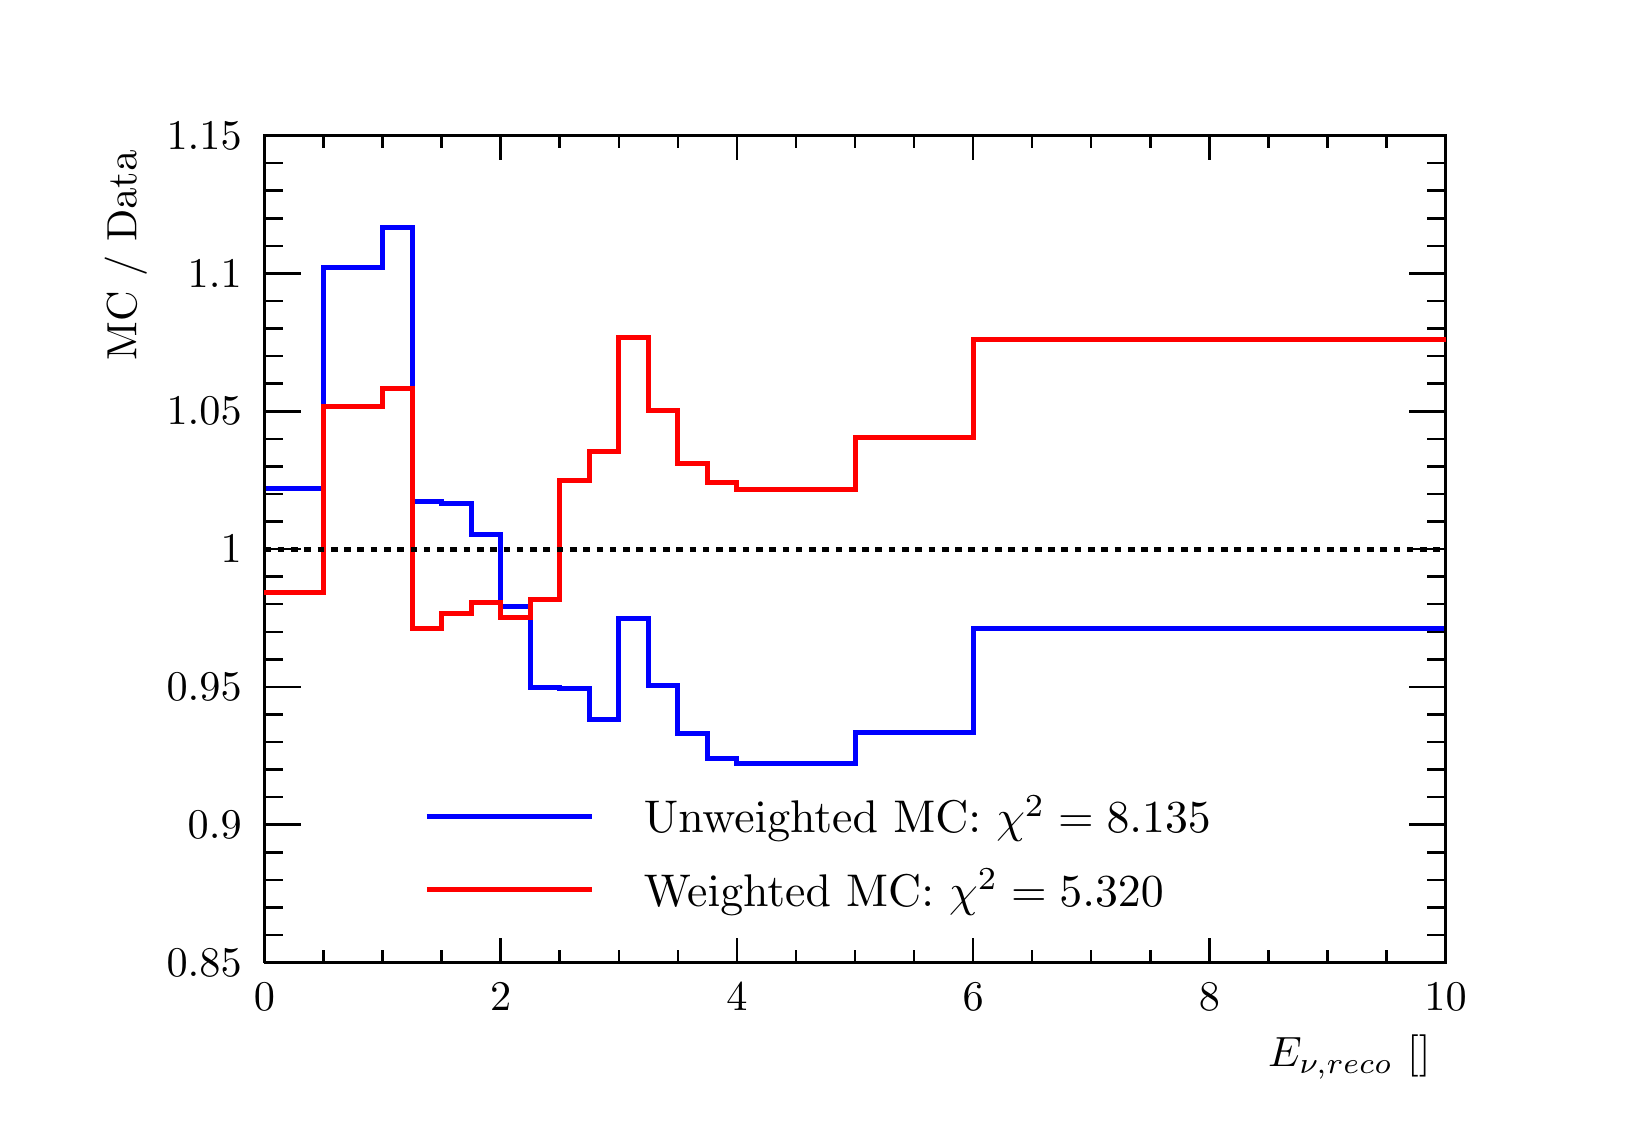
\begin{tikzpicture}
\pgfdeclareplotmark{cross} {
\pgfpathmoveto{\pgfpoint{-0.3\pgfplotmarksize}{\pgfplotmarksize}}
\pgfpathlineto{\pgfpoint{+0.3\pgfplotmarksize}{\pgfplotmarksize}}
\pgfpathlineto{\pgfpoint{+0.3\pgfplotmarksize}{0.3\pgfplotmarksize}}
\pgfpathlineto{\pgfpoint{+1\pgfplotmarksize}{0.3\pgfplotmarksize}}
\pgfpathlineto{\pgfpoint{+1\pgfplotmarksize}{-0.3\pgfplotmarksize}}
\pgfpathlineto{\pgfpoint{+0.3\pgfplotmarksize}{-0.3\pgfplotmarksize}}
\pgfpathlineto{\pgfpoint{+0.3\pgfplotmarksize}{-1.\pgfplotmarksize}}
\pgfpathlineto{\pgfpoint{-0.3\pgfplotmarksize}{-1.\pgfplotmarksize}}
\pgfpathlineto{\pgfpoint{-0.3\pgfplotmarksize}{-0.3\pgfplotmarksize}}
\pgfpathlineto{\pgfpoint{-1.\pgfplotmarksize}{-0.3\pgfplotmarksize}}
\pgfpathlineto{\pgfpoint{-1.\pgfplotmarksize}{0.3\pgfplotmarksize}}
\pgfpathlineto{\pgfpoint{-0.3\pgfplotmarksize}{0.3\pgfplotmarksize}}
\pgfpathclose
\pgfusepathqstroke
}
\pgfdeclareplotmark{cross*} {
\pgfpathmoveto{\pgfpoint{-0.3\pgfplotmarksize}{\pgfplotmarksize}}
\pgfpathlineto{\pgfpoint{+0.3\pgfplotmarksize}{\pgfplotmarksize}}
\pgfpathlineto{\pgfpoint{+0.3\pgfplotmarksize}{0.3\pgfplotmarksize}}
\pgfpathlineto{\pgfpoint{+1\pgfplotmarksize}{0.3\pgfplotmarksize}}
\pgfpathlineto{\pgfpoint{+1\pgfplotmarksize}{-0.3\pgfplotmarksize}}
\pgfpathlineto{\pgfpoint{+0.3\pgfplotmarksize}{-0.3\pgfplotmarksize}}
\pgfpathlineto{\pgfpoint{+0.3\pgfplotmarksize}{-1.\pgfplotmarksize}}
\pgfpathlineto{\pgfpoint{-0.3\pgfplotmarksize}{-1.\pgfplotmarksize}}
\pgfpathlineto{\pgfpoint{-0.3\pgfplotmarksize}{-0.3\pgfplotmarksize}}
\pgfpathlineto{\pgfpoint{-1.\pgfplotmarksize}{-0.3\pgfplotmarksize}}
\pgfpathlineto{\pgfpoint{-1.\pgfplotmarksize}{0.3\pgfplotmarksize}}
\pgfpathlineto{\pgfpoint{-0.3\pgfplotmarksize}{0.3\pgfplotmarksize}}
\pgfpathclose
\pgfusepathqfillstroke
}
\pgfdeclareplotmark{newstar} {
\pgfpathmoveto{\pgfqpoint{0pt}{\pgfplotmarksize}}
\pgfpathlineto{\pgfqpointpolar{44}{0.5\pgfplotmarksize}}
\pgfpathlineto{\pgfqpointpolar{18}{\pgfplotmarksize}}
\pgfpathlineto{\pgfqpointpolar{-20}{0.5\pgfplotmarksize}}
\pgfpathlineto{\pgfqpointpolar{-54}{\pgfplotmarksize}}
\pgfpathlineto{\pgfqpointpolar{-90}{0.5\pgfplotmarksize}}
\pgfpathlineto{\pgfqpointpolar{234}{\pgfplotmarksize}}
\pgfpathlineto{\pgfqpointpolar{198}{0.5\pgfplotmarksize}}
\pgfpathlineto{\pgfqpointpolar{162}{\pgfplotmarksize}}
\pgfpathlineto{\pgfqpointpolar{134}{0.5\pgfplotmarksize}}
\pgfpathclose
\pgfusepathqstroke
}
\pgfdeclareplotmark{newstar*} {
\pgfpathmoveto{\pgfqpoint{0pt}{\pgfplotmarksize}}
\pgfpathlineto{\pgfqpointpolar{44}{0.5\pgfplotmarksize}}
\pgfpathlineto{\pgfqpointpolar{18}{\pgfplotmarksize}}
\pgfpathlineto{\pgfqpointpolar{-20}{0.5\pgfplotmarksize}}
\pgfpathlineto{\pgfqpointpolar{-54}{\pgfplotmarksize}}
\pgfpathlineto{\pgfqpointpolar{-90}{0.5\pgfplotmarksize}}
\pgfpathlineto{\pgfqpointpolar{234}{\pgfplotmarksize}}
\pgfpathlineto{\pgfqpointpolar{198}{0.5\pgfplotmarksize}}
\pgfpathlineto{\pgfqpointpolar{162}{\pgfplotmarksize}}
\pgfpathlineto{\pgfqpointpolar{134}{0.5\pgfplotmarksize}}
\pgfpathclose
\pgfusepathqfillstroke
}
\definecolor{c}{rgb}{1,1,1};
\draw [color=c, fill=c] (0,0) rectangle (20,13.639);
\draw [color=c, fill=c] (3,1.77307) rectangle (18,12.2751);
\definecolor{c}{rgb}{0,0,0};
\draw [c,line width=0.9] (3,1.77307) -- (3,12.2751) -- (18,12.2751) -- (18,1.77307) -- (3,1.77307);
\definecolor{c}{rgb}{1,1,1};
\draw [color=c, fill=c] (3,1.77307) rectangle (18,12.2751);
\definecolor{c}{rgb}{0,0,0};
\draw [c,line width=0.9] (3,1.77307) -- (3,12.2751) -- (18,12.2751) -- (18,1.77307) -- (3,1.77307);
\definecolor{c}{rgb}{0,0,1};
\draw [c,line width=1.8] (3,7.79132) -- (3.75,7.79132) -- (3.75,10.5979) -- (4.5,10.5979) -- (4.5,11.1026) -- (4.875,11.1026) -- (4.875,7.62238) -- (5.25,7.62238) -- (5.25,7.59801) -- (5.625,7.59801) -- (5.625,7.214) -- (6,7.214) -- (6,6.28914) --
 (6.375,6.28914) -- (6.375,5.26513) -- (6.75,5.26513) -- (6.75,5.25813) -- (7.125,5.25813) -- (7.125,4.86413) -- (7.5,4.86413) -- (7.5,6.14598) -- (7.875,6.14598) -- (7.875,5.28572) -- (8.25,5.28572) -- (8.25,4.67637) -- (8.625,4.67637) --
 (8.625,4.37007) -- (9,4.37007) -- (9,4.30168) -- (10.5,4.30168) -- (10.5,4.69347) -- (12,4.69347) -- (12,6.01994) -- (18,6.01994);
\definecolor{c}{rgb}{0,0,0};
\draw [c,line width=0.9] (3,1.77307) -- (18,1.77307);
\draw [c,line width=0.9] (3,2.07994) -- (3,1.77307);
\draw [c,line width=0.9] (3.75,1.9265) -- (3.75,1.77307);
\draw [c,line width=0.9] (4.5,1.9265) -- (4.5,1.77307);
\draw [c,line width=0.9] (5.25,1.9265) -- (5.25,1.77307);
\draw [c,line width=0.9] (6,2.07994) -- (6,1.77307);
\draw [c,line width=0.9] (6.75,1.9265) -- (6.75,1.77307);
\draw [c,line width=0.9] (7.5,1.9265) -- (7.5,1.77307);
\draw [c,line width=0.9] (8.25,1.9265) -- (8.25,1.77307);
\draw [c,line width=0.9] (9,2.07994) -- (9,1.77307);
\draw [c,line width=0.9] (9.75,1.9265) -- (9.75,1.77307);
\draw [c,line width=0.9] (10.5,1.9265) -- (10.5,1.77307);
\draw [c,line width=0.9] (11.25,1.9265) -- (11.25,1.77307);
\draw [c,line width=0.9] (12,2.07994) -- (12,1.77307);
\draw [c,line width=0.9] (12.75,1.9265) -- (12.75,1.77307);
\draw [c,line width=0.9] (13.5,1.9265) -- (13.5,1.77307);
\draw [c,line width=0.9] (14.25,1.9265) -- (14.25,1.77307);
\draw [c,line width=0.9] (15,2.07994) -- (15,1.77307);
\draw [c,line width=0.9] (15.75,1.9265) -- (15.75,1.77307);
\draw [c,line width=0.9] (16.5,1.9265) -- (16.5,1.77307);
\draw [c,line width=0.9] (17.25,1.9265) -- (17.25,1.77307);
\draw [c,line width=0.9] (18,2.07994) -- (18,1.77307);
\draw [anchor=base] (3,1.15931) node[scale=1.52731, color=c, rotate=0]{0};
\draw [anchor=base] (6,1.15931) node[scale=1.52731, color=c, rotate=0]{2};
\draw [anchor=base] (9,1.15931) node[scale=1.52731, color=c, rotate=0]{4};
\draw [anchor=base] (12,1.15931) node[scale=1.52731, color=c, rotate=0]{6};
\draw [anchor=base] (15,1.15931) node[scale=1.52731, color=c, rotate=0]{8};
\draw [anchor=base] (18,1.15931) node[scale=1.52731, color=c, rotate=0]{10};
\draw [anchor= east] (18,0.572837) node[scale=1.52731, color=c, rotate=0]{$E_{\nu, \text{reco}}$ [\si{\GeV}] };
\draw [c,line width=0.9] (3,12.2751) -- (18,12.2751);
\draw [c,line width=0.9] (3,11.9682) -- (3,12.2751);
\draw [c,line width=0.9] (3.75,12.1216) -- (3.75,12.2751);
\draw [c,line width=0.9] (4.5,12.1216) -- (4.5,12.2751);
\draw [c,line width=0.9] (5.25,12.1216) -- (5.25,12.2751);
\draw [c,line width=0.9] (6,11.9682) -- (6,12.2751);
\draw [c,line width=0.9] (6.75,12.1216) -- (6.75,12.2751);
\draw [c,line width=0.9] (7.5,12.1216) -- (7.5,12.2751);
\draw [c,line width=0.9] (8.25,12.1216) -- (8.25,12.2751);
\draw [c,line width=0.9] (9,11.9682) -- (9,12.2751);
\draw [c,line width=0.9] (9.75,12.1216) -- (9.75,12.2751);
\draw [c,line width=0.9] (10.5,12.1216) -- (10.5,12.2751);
\draw [c,line width=0.9] (11.25,12.1216) -- (11.25,12.2751);
\draw [c,line width=0.9] (12,11.9682) -- (12,12.2751);
\draw [c,line width=0.9] (12.75,12.1216) -- (12.75,12.2751);
\draw [c,line width=0.9] (13.5,12.1216) -- (13.5,12.2751);
\draw [c,line width=0.9] (14.25,12.1216) -- (14.25,12.2751);
\draw [c,line width=0.9] (15,11.9682) -- (15,12.2751);
\draw [c,line width=0.9] (15.75,12.1216) -- (15.75,12.2751);
\draw [c,line width=0.9] (16.5,12.1216) -- (16.5,12.2751);
\draw [c,line width=0.9] (17.25,12.1216) -- (17.25,12.2751);
\draw [c,line width=0.9] (18,11.9682) -- (18,12.2751);
\draw [c,line width=0.9] (3,1.77307) -- (3,12.2751);
\draw [c,line width=0.9] (3.462,1.77307) -- (3,1.77307);
\draw [c,line width=0.9] (3.231,2.12313) -- (3,2.12313);
\draw [c,line width=0.9] (3.231,2.4732) -- (3,2.4732);
\draw [c,line width=0.9] (3.231,2.82327) -- (3,2.82327);
\draw [c,line width=0.9] (3.231,3.17333) -- (3,3.17333);
\draw [c,line width=0.9] (3.462,3.5234) -- (3,3.5234);
\draw [c,line width=0.9] (3.231,3.87347) -- (3,3.87347);
\draw [c,line width=0.9] (3.231,4.22353) -- (3,4.22353);
\draw [c,line width=0.9] (3.231,4.5736) -- (3,4.5736);
\draw [c,line width=0.9] (3.231,4.92367) -- (3,4.92367);
\draw [c,line width=0.9] (3.462,5.27373) -- (3,5.27373);
\draw [c,line width=0.9] (3.231,5.6238) -- (3,5.6238);
\draw [c,line width=0.9] (3.231,5.97387) -- (3,5.97387);
\draw [c,line width=0.9] (3.231,6.32394) -- (3,6.32394);
\draw [c,line width=0.9] (3.231,6.674) -- (3,6.674);
\draw [c,line width=0.9] (3.462,7.02407) -- (3,7.02407);
\draw [c,line width=0.9] (3.231,7.37414) -- (3,7.37414);
\draw [c,line width=0.9] (3.231,7.7242) -- (3,7.7242);
\draw [c,line width=0.9] (3.231,8.07427) -- (3,8.07427);
\draw [c,line width=0.9] (3.231,8.42434) -- (3,8.42434);
\draw [c,line width=0.9] (3.462,8.7744) -- (3,8.7744);
\draw [c,line width=0.9] (3.231,9.12447) -- (3,9.12447);
\draw [c,line width=0.9] (3.231,9.47454) -- (3,9.47454);
\draw [c,line width=0.9] (3.231,9.8246) -- (3,9.8246);
\draw [c,line width=0.9] (3.231,10.1747) -- (3,10.1747);
\draw [c,line width=0.9] (3.462,10.5247) -- (3,10.5247);
\draw [c,line width=0.9] (3.231,10.8748) -- (3,10.8748);
\draw [c,line width=0.9] (3.231,11.2249) -- (3,11.2249);
\draw [c,line width=0.9] (3.231,11.5749) -- (3,11.5749);
\draw [c,line width=0.9] (3.231,11.925) -- (3,11.925);
\draw [c,line width=0.9] (3.462,12.2751) -- (3,12.2751);
\draw [c,line width=0.9] (3.462,1.77307) -- (3,1.77307);
\draw [c,line width=0.9] (3.462,12.2751) -- (3,12.2751);
\draw [anchor= east] (2.9,1.77307) node[scale=1.52731, color=c, rotate=0]{0.85};
\draw [anchor= east] (2.9,3.5234) node[scale=1.52731, color=c, rotate=0]{0.9};
\draw [anchor= east] (2.9,5.27373) node[scale=1.52731, color=c, rotate=0]{0.95};
\draw [anchor= east] (2.9,7.02407) node[scale=1.52731, color=c, rotate=0]{1};
\draw [anchor= east] (2.9,8.7744) node[scale=1.52731, color=c, rotate=0]{1.05};
\draw [anchor= east] (2.9,10.5247) node[scale=1.52731, color=c, rotate=0]{1.1};
\draw [anchor= east] (2.9,12.2751) node[scale=1.52731, color=c, rotate=0]{1.15};
\draw [anchor= east] (1.24,12.2751) node[scale=1.52731, color=c, rotate=90]{MC / Data};
\draw [c,line width=0.9] (18,1.77307) -- (18,12.2751);
\draw [c,line width=0.9] (17.538,1.77307) -- (18,1.77307);
\draw [c,line width=0.9] (17.769,2.12313) -- (18,2.12313);
\draw [c,line width=0.9] (17.769,2.4732) -- (18,2.4732);
\draw [c,line width=0.9] (17.769,2.82327) -- (18,2.82327);
\draw [c,line width=0.9] (17.769,3.17333) -- (18,3.17333);
\draw [c,line width=0.9] (17.538,3.5234) -- (18,3.5234);
\draw [c,line width=0.9] (17.769,3.87347) -- (18,3.87347);
\draw [c,line width=0.9] (17.769,4.22353) -- (18,4.22353);
\draw [c,line width=0.9] (17.769,4.5736) -- (18,4.5736);
\draw [c,line width=0.9] (17.769,4.92367) -- (18,4.92367);
\draw [c,line width=0.9] (17.538,5.27373) -- (18,5.27373);
\draw [c,line width=0.9] (17.769,5.6238) -- (18,5.6238);
\draw [c,line width=0.9] (17.769,5.97387) -- (18,5.97387);
\draw [c,line width=0.9] (17.769,6.32394) -- (18,6.32394);
\draw [c,line width=0.9] (17.769,6.674) -- (18,6.674);
\draw [c,line width=0.9] (17.538,7.02407) -- (18,7.02407);
\draw [c,line width=0.9] (17.769,7.37414) -- (18,7.37414);
\draw [c,line width=0.9] (17.769,7.7242) -- (18,7.7242);
\draw [c,line width=0.9] (17.769,8.07427) -- (18,8.07427);
\draw [c,line width=0.9] (17.769,8.42434) -- (18,8.42434);
\draw [c,line width=0.9] (17.538,8.7744) -- (18,8.7744);
\draw [c,line width=0.9] (17.769,9.12447) -- (18,9.12447);
\draw [c,line width=0.9] (17.769,9.47454) -- (18,9.47454);
\draw [c,line width=0.9] (17.769,9.8246) -- (18,9.8246);
\draw [c,line width=0.9] (17.769,10.1747) -- (18,10.1747);
\draw [c,line width=0.9] (17.538,10.5247) -- (18,10.5247);
\draw [c,line width=0.9] (17.769,10.8748) -- (18,10.8748);
\draw [c,line width=0.9] (17.769,11.2249) -- (18,11.2249);
\draw [c,line width=0.9] (17.769,11.5749) -- (18,11.5749);
\draw [c,line width=0.9] (17.769,11.925) -- (18,11.925);
\draw [c,line width=0.9] (17.538,12.2751) -- (18,12.2751);
\draw [c,line width=0.9] (17.538,1.77307) -- (18,1.77307);
\draw [c,line width=0.9] (17.538,12.2751) -- (18,12.2751);
\definecolor{c}{rgb}{1,0,0};
\draw [c,line width=1.8] (3,6.46772) -- (3.75,6.46772) -- (3.75,8.8383) -- (4.5,8.8383) -- (4.5,9.06288) -- (4.875,9.06288) -- (4.875,6.01024) -- (5.25,6.01024) -- (5.25,6.20955) -- (5.625,6.20955) -- (5.625,6.35137) -- (6,6.35137) -- (6,6.15732) --
 (6.375,6.15732) -- (6.375,6.38792) -- (6.75,6.38792) -- (6.75,7.89712) -- (7.125,7.89712) -- (7.125,8.2613) -- (7.5,8.2613) -- (7.5,9.71673) -- (7.875,9.71673) -- (7.875,8.78869) -- (8.25,8.78869) -- (8.25,8.11626) -- (8.625,8.11626) --
 (8.625,7.86632) -- (9,7.86632) -- (9,7.77864) -- (10.5,7.77864) -- (10.5,8.44243) -- (12,8.44243) -- (12,9.68059) -- (18,9.68059);
\definecolor{c}{rgb}{0,0,0};
\draw [c,dash pattern=on 2.40pt off 2.40pt ,line width=1.8] (3,7.02407) -- (18,7.02407);
\definecolor{c}{rgb}{1,1,1};
\draw [color=c, fill=c] (4.61318,2.23496) rectangle (16.6189,4.09742);
\definecolor{c}{rgb}{0,0,0};
\draw [anchor=base west] (7.61461,3.42228) node[scale=1.65459, color=c, rotate=0]{Unweighted MC: $\chi^{2} = 8.135$};
\definecolor{c}{rgb}{0,0,1};
\draw [c,line width=1.8] (5.0634,3.63181) -- (7.1644,3.63181);
\definecolor{c}{rgb}{0,0,0};
\draw [anchor=base west] (7.61461,2.49105) node[scale=1.65459, color=c, rotate=0]{Weighted MC: $\chi^{2} = 5.320$};
\definecolor{c}{rgb}{1,0,0};
\draw [c,line width=1.8] (5.0634,2.70057) -- (7.1644,2.70057);
\definecolor{c}{rgb}{1,1,1};
\draw [color=c, fill=c] (2,12.8206) rectangle (18,13.5708);
\definecolor{c}{rgb}{0,0,0};
%\draw (10,13.1957) node[scale=1.40004, color=c, rotate=0]{Unweighted MC};
\end{tikzpicture}
